%!TEX root = ../thesis.tex

\chapter{理论模型}
综合 \ref{sec:zs} 中各学者的观点,以及现实中的违约案例,本文将从宏观、中观以及微观角度,拆解可能影响违约的因素。
\section{微观层次}
本文将微观层面影响企业违约的因素分为以下四类,主要包含企业级的指标:
\subsection{公司层面}

国企发行了80\%的债券,但违约中只占了15\%,有学者指出可能是由于国企存在政府支持\cite{mo2021china},也有可能国企通常相对资金雄厚,经营情况较好。因此,本文将公司性质作为影响因素之一建模。
同样的,上市企业比非上市企业融资方式更多,融资额往往也更大,部分违约企业也将自我总结违约原因是上市失败,因此上市与否或许也可能影响违约。

股东对企业的支持也可能影响是否违约,如苏宁易购缺乏实控人,在企业危难时各股东自扫门前雪,没有人向企业注血,最终苏宁走向违约。通常而言大股东持股比例越高,对企业的重视程度会越大,更有可能为了避免违约后其持有的大量股权价值归零而为企业提供资金支持或豁免债务。

此外,正如\ref{sec:zs}中众多学者对公司治理的研究所揭示,公司治理成效也可能影响违约因素。
但是一方面公司治理会影响违约与否,另一方面违约企业通常会面临法律纠纷、债权人接管等情况,令企业公司治理发生很大变化。本文计划以持有基金占比作为公司治理的代理变量。
公募基金虽然会考虑违约与否,但更加担心债券持有期间贬值。
公募基金持有债券类似于交易性金融资产,买入的目的可以是获得利息收入或者未来得到债券估值的资本利得;而银行持有债券交易更少,等待还本付息,类似于持有至到期投资。
公募基金在评级下调超出风控阈值后必须斩仓,即便债券因流动性过低有价无市,而所有违约债券都或迟或早会被下调为垃圾级,但评级下调的债券中违约中终究只是少数,因此公募基金持有比例与违约弱相关。
公募基金更多是扮演财务投资者的角色由于担心债券在持有期间贬值,这就使他们更加会担心企业公司治理存在问题。如果公司治理水平低,债券潜在的下跌可能性更大\Parencite{anginer2018corporate}。即基金持有比例和公司治理强相关。
因此本文计划采用基金持有比例来表征公司治理。

最后,公司层面还有一些难以量化到因素,如发行人主观意愿(花样年地产账面现金充足“花式”躺平违约)、财务造假(康美药业、五洋建设)。但因此违约的终是少数,绝大多数地产商苦苦挣扎避免躺平,绝大多数企业报表准确。因此本文不将这些因素纳入考虑。
\subsection{经营层面}
企业面临流动性危机,很多情况下是经营不及预期,营收大幅亏损,如原超日太阳在连续三年大额亏损后,最终无法兑付利息成为打破刚兑的第一例违约。

客户集中度过高,可能会导致企业面临较高的风险\cite{王雄元2017客户集中度与公司债二级市场信用利差}。集中的客户有能力要求企业降价、使用商票结算等以降低自身成本,通过压迫企业获得更大利润空间。例如建设承包商南通三建持有大量恒大商票得不到兑付,不得不寻求债务展期。

经营过程中的杠杆率也有可能影响违约\cite{王永钦2019杠杆率如何影响资产价格},如以“高杠杆-高周转”著称的恒大,在融资受限时高杠杆的游戏进行不下去。但一方面很多违约公司会美化负债率,用诸如战略投资者等明股实债的方式,用尽各种手段将负债隐藏到表外;另一方面,不同性质的行业杠杆差异较大,如重工业和服务业之间相似的负债率并不意味着相近的爆仓的可能性,简单的比较负债率并不可取。基于此本文不采用资产负债表科目刻画杠杆率,而是采用标准券折算率这一比较市场化的指标,即质押企业债券可以获得多大比例的标准券来衡量企业杠杆率。折算率高意味着市场允许企业可以通过质押债券的方式撬动更多融资,市场允许其加更高的杠杆。且折算率对于优质企业有上限,对于违约风险更大的企业更敏感。

\subsection{财务层面}
对于会计指标,\Textcite{blochlinger2018ratings}指出 Altman's Z 指标是一个比较综合的、很好的预测违约会计指标。
此外违约本质上是企业持有的现金及其等价物无法偿还到期债务,存在一定的可能公司真的遇到了短期流动性危机而未来长期表现将会王者归来,如盐湖股份,因此本文也将考虑现金短债比这一因素。
\subsection{评级指标}
\ref{sec:zs} 中各学者对评级指标的批判非常有借鉴意义。但即便以预测的角度看评级并不完全准确,但以后验的角度看,评级也反映了一定的公开与非公开信息,因此本文也将主体评级纳入考虑。
\section{中观层次}
中观层次为非企业级、非全国级的因素。如行业、流动性和地理因素。

\begin{figure}[h]
	\centering
	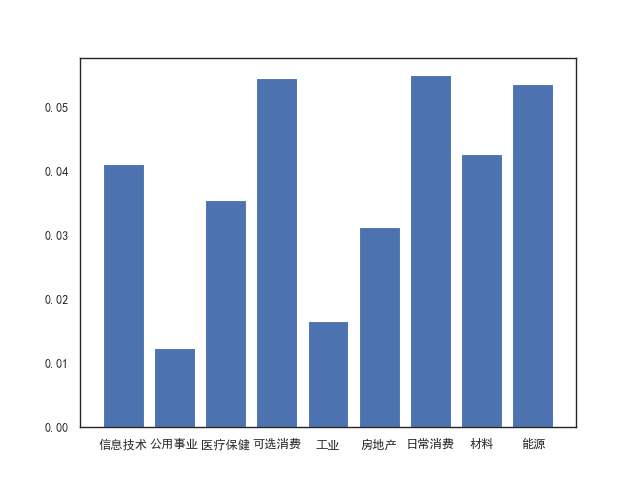
\includegraphics[width=.9\linewidth]{./data/industry.png}
	\caption{\label{fig:industry}违约债分行业分布}
\end{figure}

如表 \ref{fig:industry} 所示,看似较高违约率的行业,
均是因为单一主体违约余额较大(如方正集团导致计算机行业、华晨汽车导致汽车行业、紫光集团导致电子行业、山东如意导致纺织行业违约率激增)。如国外的情况\cite{azizpour2018exploring},我国债券违约亦基本可以排除大多数的行业聚类,即某行业因行业景气集中某段时间违约的情况。即便是近期的房地产违约风波,也并非主要由于行业景气度,而是由于房地产“三条红线”等政策约束高杠杆的经营。因此本文将主要考虑房地产政策(房地产行业且时间大于 2020 年),而不考虑每个行业本身。

\begin{figure}[h]
	\centering
	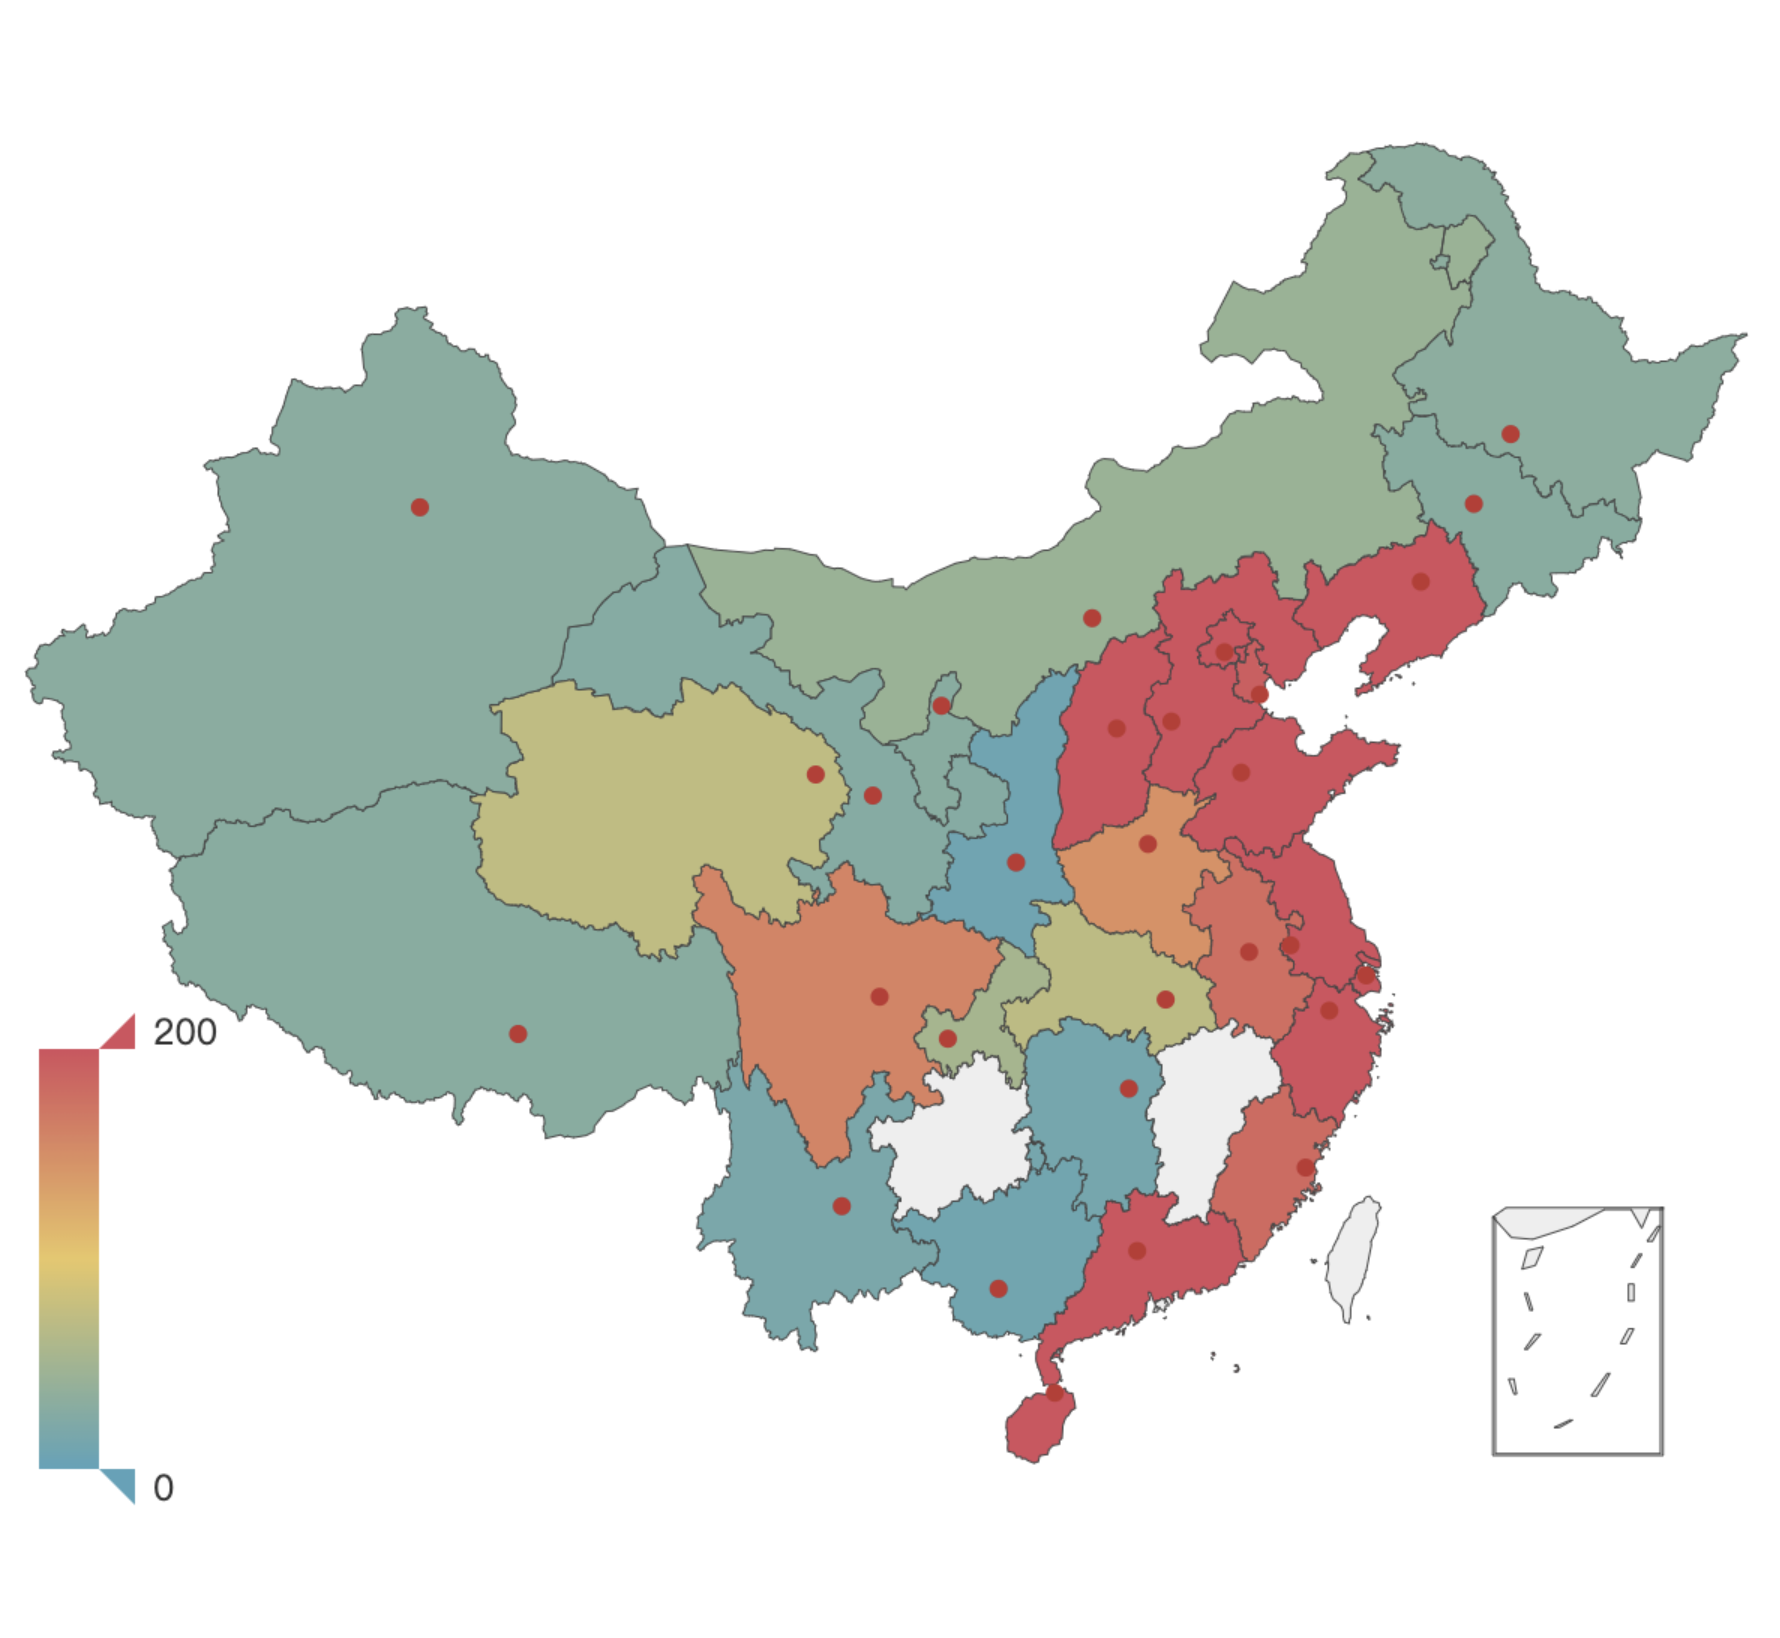
\includegraphics[width=.9\linewidth]{./data/default_by_geo.png}
	\caption{\label{fig:geo}违约债地理分布}
\end{figure}
地理上看,
一方面经济落后地区违约风险较大,一方面经济较好的地区企业发债数量较多可能导致违约金额较大,如图\ref{fig:geo}显示出后一种作用较强,尽管某些经济欠发达地区似乎仍然维持刚性兑付。尽管看似部分地区违约率高,但事实上高违约率的原因大多也是单一违约主体违约金额大,如河北的华夏幸福、辽宁的华晨宝马、海南的海航、青海的青国投等等,总的来说地理上的传染尚不明晰。

最后是流动性,本文计划以市场成交金额为流动性指标。当市场流动性偏紧时,如永煤违约后风险偏好迅速下降,各机构连 AAA 国企也不敢买,成交量萎靡流动性偏紧,进而导致一级市场上冀中能源、紫光、清华控股等无法发债接续,到期压力巨大,最终部分企业走向违约。
\section{宏观层次}
如\ref{sec:zs}中学者研究,货币政策与财政政策可能会对企业违约有影响。本文计划财政政策使用政府支出占GDP比重表征,货币政策以 SHIBOR 利率表征。

有学者对债券回报率做 Fama 因子分析
\cite{chung2019volatility}
,发现以 VIX 指数为代表的波动风险的影响是普遍存在的。
因此本文效仿选择上证 50 期权的隐含波动率作为波动率指标,2015 年期权推出之前则采用上证历史波动率。
